\chapter{Theoretical Background}

This chapter will give a brief overview about the underlying theoretical background in the fields of antenna theory, spatial sampling and will introduce some methods of integration to derive the \ac{TRP} out of spherical \ac{EIRP}-data.

\section{Antenna Field Regions}

\begin{figure}[H]
\centering
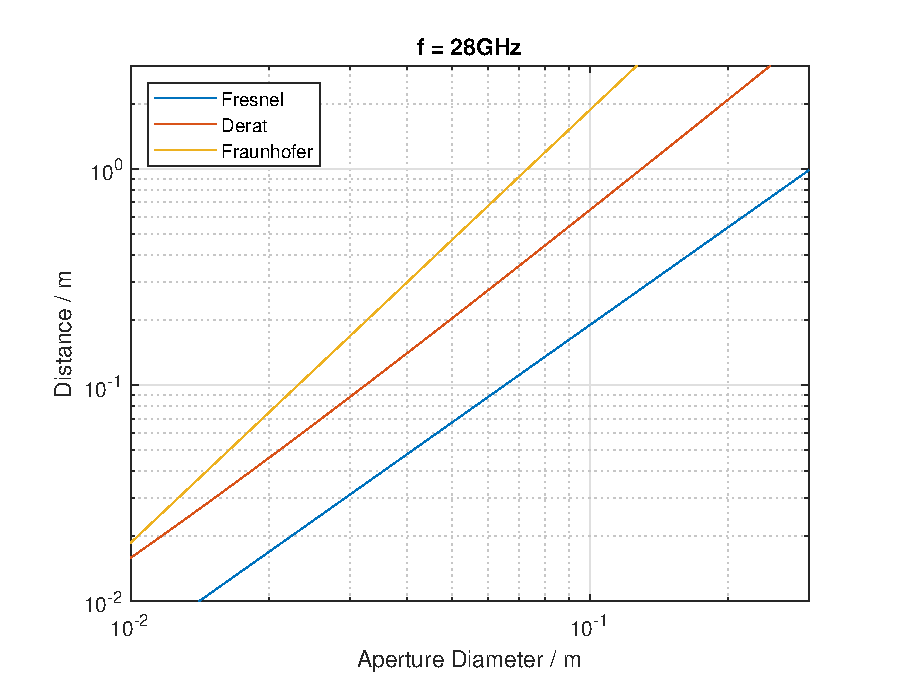
\includegraphics[width=0.6\textwidth]{Matlab/AntennaFieldRegions.eps}
\caption{Antenna field regions overview}
\label{fig:antennafieldreg}
\end{figure}

There are three commonly known antenna regions, the reactive \ac{NF}, the radiating \ac{NF} and the \ac{FF}, divided by tow boundaries, the Fresnel distance (blue) and the Fraunhofer distance (yellow). These distances are shown in figure \ref{fig:antennafieldreg}, where the aperture diameter of an arbitrary antenna is on the x-axis and the distance form it is on the y-axis. The third line, the Derat distance (red) was introduced by Benoit Derat. \cite{8393926} All distances will be explained in the following.\\
\ac{FF}-distance and \ac{NF}-distance are derivable from the phase fluctuation due to the maximum diameter of the antennas aperture \cite{7942128} in a distance $r$ from the antennas phase center. The phase fluctuation is given by the different length of $r$ and $R$, as you can see in figure \ref{fig:arbaperturexy}. The maximum runtime difference is found at the minimum radius of the circle enclosing the aperture at $\sfrac{D}{2}$. The field boundaries are derived from the Taylor series of the function of the phase in dot $P$. Fresnel and Fraunhofer distance, the boundaries between reactive \ac{NF}, radiating \ac{NF} (Fresnel-Region) and the \ac{FF} (Fraunhofer-Region), are analogue to their optical counterpart. \cite{7942128} \cite{balanis}

\begin{figure}[H]
\centering
\def\svgwidth{0.6\textwidth}
\input{Bilder/AntennaApature.pdf_tex}
\caption{An arbitrary radiating aperture in the $yz$ plane. \cite{7942128}}
\label{fig:arbaperturexy}
\end{figure}

$R$ can be written as: \cite{balanis}

\begin{equation}
R = \sqrt{\left(x^2+y^2+z^2\right)-\left(2zz'-z^{\prime\, 2}\right)}=\sqrt{r^2-\left(2rz'\sin \theta -z^{\prime\, 2}\right)}
\end{equation}

Using the binomial expansion, $R$ can be written as:

\begin{equation}
R = r - z'\sin\theta + \frac{1}{r}\left(\frac{z^{\prime\, 2}}{2}\cos ^2 \theta\right) + \frac{1}{r^2}\left(\frac{z^{\prime\, 3}}{2}\sin\theta\cos^2\theta\right) + \dots
\end{equation}

\subsection{Far-Field}

According to \cite{balanis} the \ac{FF}-distance is \glqq that region of the field of an antenna where the angular field distribution is essentially independent of the distance from the antenna.\grqq{ }That means that the antennas pattern is mostly independent from the distance to the antenna.\\
For the \ac{FF} assumption it is convenient to use the two most significant terms of the binomial expansion $R\approx r - z'\sin\theta$. Hence the error of that truncation can be expressed as the maximum of the third most significant term:

\begin{equation}
\frac{1}{r}\left(\frac{z^{\prime\, 2}}{2}\cos ^2 \theta\right)_\text{max} = \frac{z^{\prime\, 2}}{2r} \quad , \quad \theta = 0
\label{eq:dphi1}
\end{equation}

Introducing the angular wavenumber $k=\sfrac{2\pi}{\lambda}$ and $z'=\sfrac{D}{2}$, formula \ref{eq:dphi1} can be written as:


\begin{equation}
\Delta\phi = \frac{k\cdot z^{\prime\, 2}}{2r} =\frac{\frac{2\pi}{\lambda}\cdot \left(\frac{D}{2}\right)^2}{2r} = \frac{\pi D^2}{4\lambda\cdot r}
\end{equation}

With the often used phase error of $\Delta\phi = \sfrac{\pi}{8} \ \widehat{=}\  22.5^\circ$ the well known \ac{FF}-distance-formula $r_{\text{Fr}}$ can be derived:

\begin{equation}
\frac{\pi}{8} = \frac{\pi D^2}{4\lambda\cdot r_{\text{Fr}}} \quad \Leftrightarrow \quad r_{\text{Fr}} = \frac{2D^2}{\lambda}
\end{equation}

This equation is valid for $D > \lambda$. \cite{balanis}

\subsection{Near-Field}

The radiating \ac{NF} (Fresnel) -region is defined \cite{balanis} as \glqq that region of the field of an antenna between the reactive near-field region and the far-field region wherein radiation fields predominate and wherein the angular field distribution is dependent upon the distance from the antenna.\grqq{ }That means that the antennas pattern is dependent from the distance to the antenna.\\
In the radiating \ac{NF} the deviation from the third most significant term is more then $\sfrac{\pi}{8}$, so it is no longer negligible. With the derivation of the next term the maximum deviation is found:

\begin{align}
\frac{\partial}{\partial\theta}\left(\frac{1}{r^2}\left(\frac{z^{\prime\, 3}}{2}\sin\theta\cos^2\theta\right)\right) = \frac{z^{\prime\, 3}}{2r^2}\cos\theta\left(\cos^2\theta-2\sin^2\theta\right) = 0 \quad \Leftrightarrow\\ 
\theta_1 = \frac{\pi}{2},\ \theta_2=2\arctan\left(\sqrt{5-2\sqrt{6}}\right) \quad \Leftrightarrow
\end{align}

By introducing the angular wavenumber $k=\sfrac{2\pi}{\lambda}$, the minimum sphere diameter $D$ that $z'=\sfrac{D}{2}$ and the phase error of $\Delta\phi = \sfrac{\pi}{8} \ \widehat{=}\  22.5^\circ$ the \ac{NF} (Fresnel)-distance-formula $r_{\text{NF}}$ can be derived:

\begin{equation}
\Delta\phi = \frac{\pi}{8} = \frac{kz^{\prime\, 3}}{2r_{\text{NF}}^2}\sin\theta_2\cos^2\theta_2= \frac{\pi D^3}{12\sqrt{3}\cdot\lambda r_{\text{NF}}^2} \quad \Leftrightarrow \quad r_{\text{NF}}=0.62\sqrt{\frac{D^3}{\lambda}}
\end{equation}

The region directly surrounding the antenna in front of this boundary is called reactive \ac{NF} and it is according to \cite{balanis} \glqq that portion of the near-field region immediately surrounding the antenna wherein the reactive field predominates.\grqq{ }In other words, the reactive \ac{NF} is that portion of an antennas field were you would expect direct coupling.

\subsection{Derat Distance}

The Derat distance was introduced by Benoit Derat in \cite{8393926} and it is that distance, in which the main beam of an antenna is in \ac{FF} condition. For the understanding of the Derat distance $r_{\text{Dr}}$ other considerations need to take place: It is about spherical modes described by spherical Hankel functions  of the second kind. \cite{8393926} \cite{hansen}\\
In \cite{8393926} it is shown, that higher order modes than 

\begin{equation}
N = \lceil 1.0252\cdot\left(\frac{\pi D}{\lambda}\right)^{0.8633} \rceil
\end{equation}

have a maximum influence to the \ac{EIRP} in main direction of $\SI{0.5}{\decibel}$. With that the Derat distance can be derived to:

\begin{equation}
r_{\text{Dr}} = \lambda\left(\frac{\pi D}{\lambda}\right)^{0.8633}\left(0.1673\left(\frac{\pi D}{\lambda}\right)^{0.8633}+0.1632\right)
\end{equation}

\subsection{Example: Standard Gain Horn}

\begin{figure}[H]
\centering
  \centering
  \subfigure[Wave impedance]{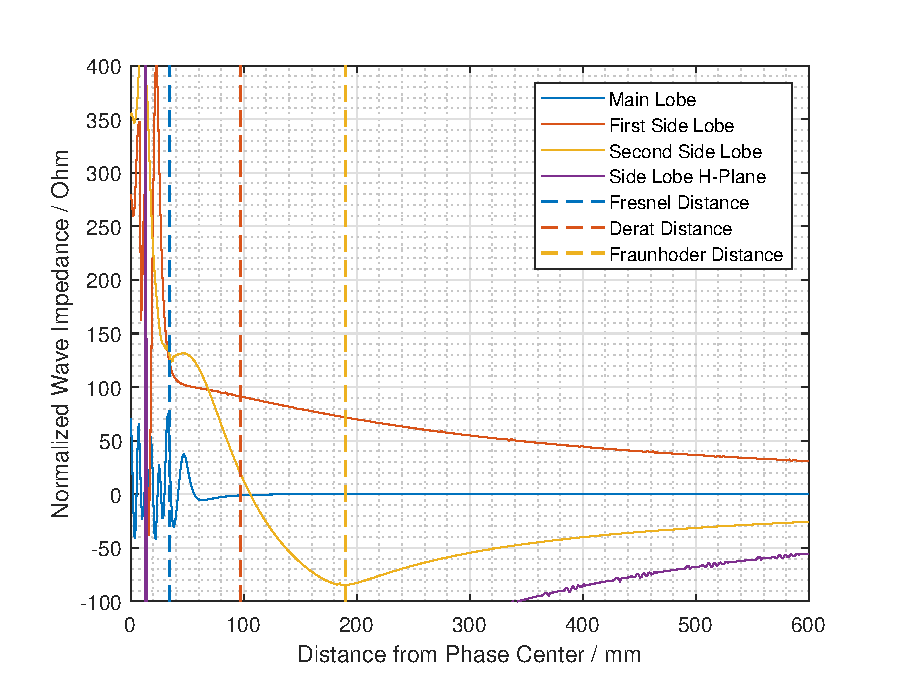
\includegraphics[width=0.49\textwidth]{Matlab/NormWaveImpHorn.eps}}
  \centering
  \subfigure[Phase]{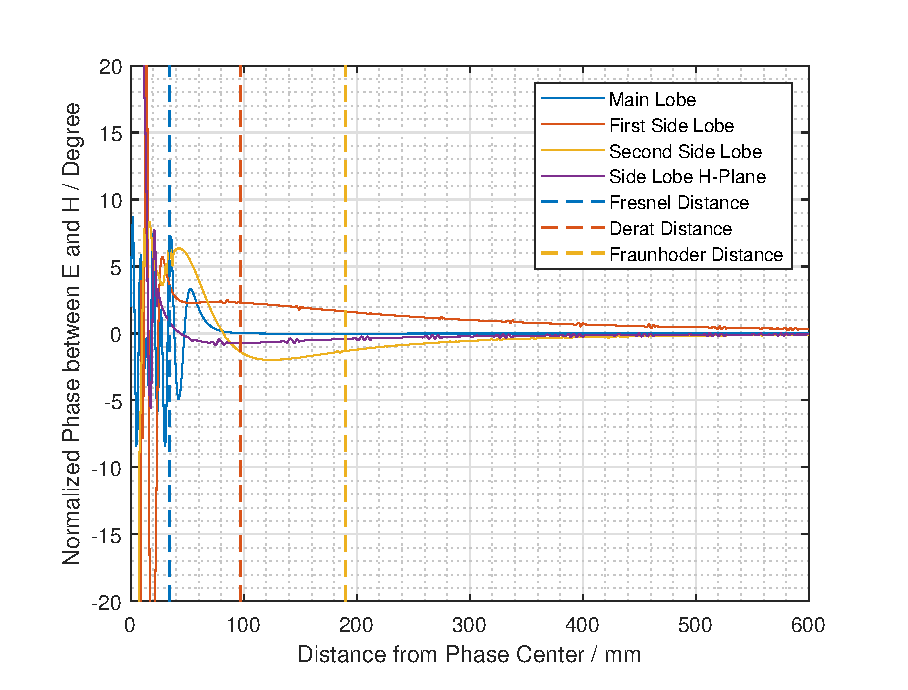
\includegraphics[width=0.49\textwidth]{Matlab/NormPhaseHorn.eps}}
  \centering
  \subfigure[Antenna Pattern E-Plane]{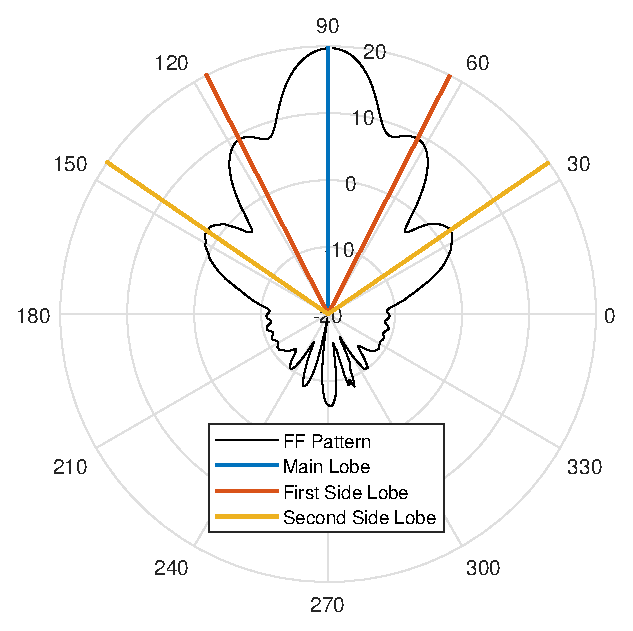
\includegraphics[width=0.3\textwidth]{Matlab/ePlanePattern.eps}}
\caption{Beam comparison of a $\SI{20}{\decibel}$ SGH at $\SI{28}{\giga\hertz}$}
\label{fig:beamcpmp}
\end{figure}

To clarify the introduced distances they will be proofed based on a $\SI{20}{\decibel}$ \ac{SGH} at $\SI{28}{\giga\hertz}$. If you look in the annex at figure \ref{fig:fielddist} you see the front view of this horn with the underlying field distribution. The polarisation is in $y$-direction, so the $yz$-plane is called E-plane and the $xz$-plane is called H-plane from here on.\\
In figure \ref{fig:beamcpmp} the normalized wave impedance (a) and the normalized phase between E- and H-field components over the distance to the phase center are plotted. To clarify the designations the directions are plotted in (c). The data has been produces by CST\texttrademark , a full wave simulation tool. Complex data in $x$, $y$, and $z$ direction was exported to Matlab\texttrademark{ } and there post processed.\\
Also the field boundaries from the sections above are plotted with dashed lines. For deriving the boundaries only the opening of the horn in the E-plane was taken to account. This is rational because the field distribution and thus the usage of the aperture is known, refer to figure \ref{fig:fielddist}. As you can see in the E-plane the aperture is fully used. But if the field distribution is unknown the smallest circle enclosing the aperture has to be taken.\\
In \ref{fig:beamcpmp} (a) the normalized wave impedance of the different angels (refer to (c)) is plotted over the distance from the antennas phase center. \ref{fig:beamcpmp} (b) shows analogue to (a) the phase between E- and H-field.\\
The main lobe (blue line) is from Derat-distance on in \ac{FF} condition. On the one hand side the wave impedance reached its endvalue of $\SI{377}{\ohm}$ and on the other hand E- and H-fields are coherent. Considering the side lobes it can be seen that in the reactive \ac{NF} the field conditions are very unstable, whereas the fields in the radiating \ac{NF} become more stable. In the \ac{FF} the field values are continually decreasing the offset from their final value.\\
In figure \ref{fig:devantennap} in the annex the resulting antenna patterns in different radii are depicted as well in Cartesian coordinates (a) as in Polar coordinates (b). The assumption 

\begin{equation}
S = \frac{E^2}{Z_0}
\end{equation}

was taken to account. At Derat distance ($\approx\SI{100}{\milli\meter}$) the error in main beam direction is about $\SI{0.5}{\decibel}$ and the antenna pattern is further evolving after the Fraunhofer distance at about $\SI{200}{\milli\meter}$.

\section{Spatial Sampling Approaches}

\begin{figure}[H]
\centering
\def\svgwidth{0.4\textwidth}
\input{Bilder/KoordinateSystem.pdf_tex}
\caption{The underling coordinate system}
\label{coordinates}
\end{figure}

In figure \ref{coordinates} the used coordinate system is depicted. In comparison with a globe the latitude is described by the elevation with the symbol $\Theta$ and the longitude is described by the azimuth with the symbol $\Phi$. The value range of $\Theta$ and $\Phi$ is:

\begin{equation}
-\frac{\pi}{2} \leq \Theta <\frac{\pi}{2}\, ,\quad -\pi \leq \Phi < \pi
\end{equation}

Hereinafter different spatial sampling approaches for this sphere are introduced. For the development of a sampling grid a sampling frequency is necessary and will be introduced in the next section.

\subsection{Derivation of the Spatial Sampling considering the Array Factor}

Ether the sampling frequency in elevation or in azimuth is depend on the aperture of the \ac{DUT} and the wavelength. To investigating the necessary sampling frequency an one dimensional $\sfrac{\lambda}{2}$ array of isotropic radiators was taken to account. With the number of elements $N$, the element spacing $d = \sfrac{\lambda}{2}$ and the wavelength $\lambda$ the antenna pattern is derivable: \cite{litze}

\begin{equation}
\begin{vmatrix}\Gamma\left(\theta\right)\end{vmatrix}^2 = \Biggl|\frac{\sin\left(\frac{\pi M d}{\lambda \sin\left(\theta\right)}\right)}{\sin\left(\frac{\pi d}{\lambda \sin\left(\theta\right)}\right)}\Biggl|^2 = \Biggl|\frac{\sin\left(\frac{\pi M}{2 \sin\left(\theta\right)}\right)}{\sin\left(\frac{\pi}{2 \sin\left(\theta\right)}\right)}\Biggl|^2
\end{equation}

\begin{figure}
  \centering
  \subfigure[Two elements: Pattern]{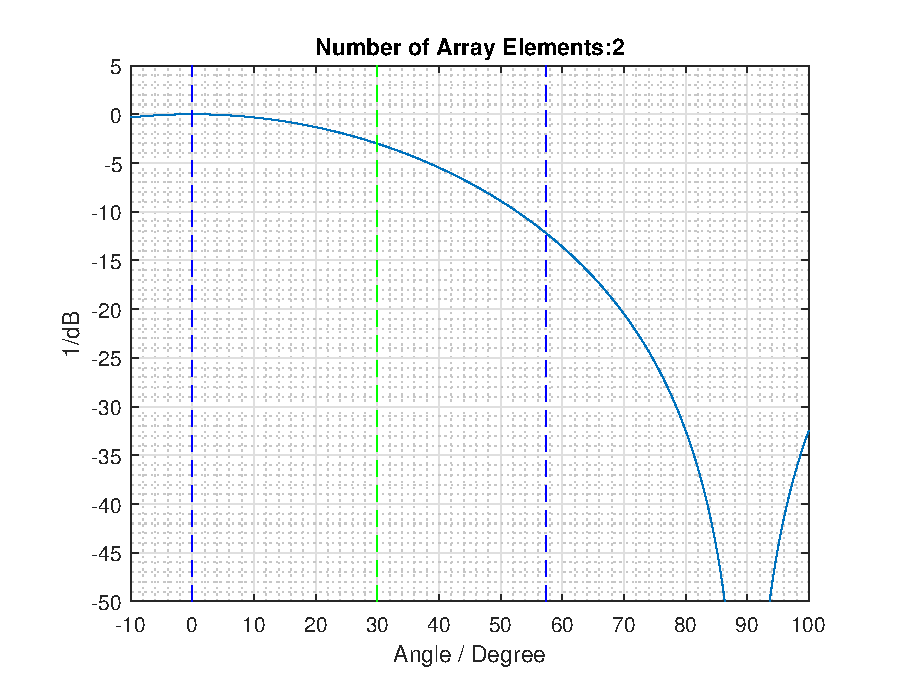
\includegraphics[width=0.32\textwidth]{Matlab/NoNumEl2.eps}}
  \centering
  \subfigure[Six elements: Pattern]{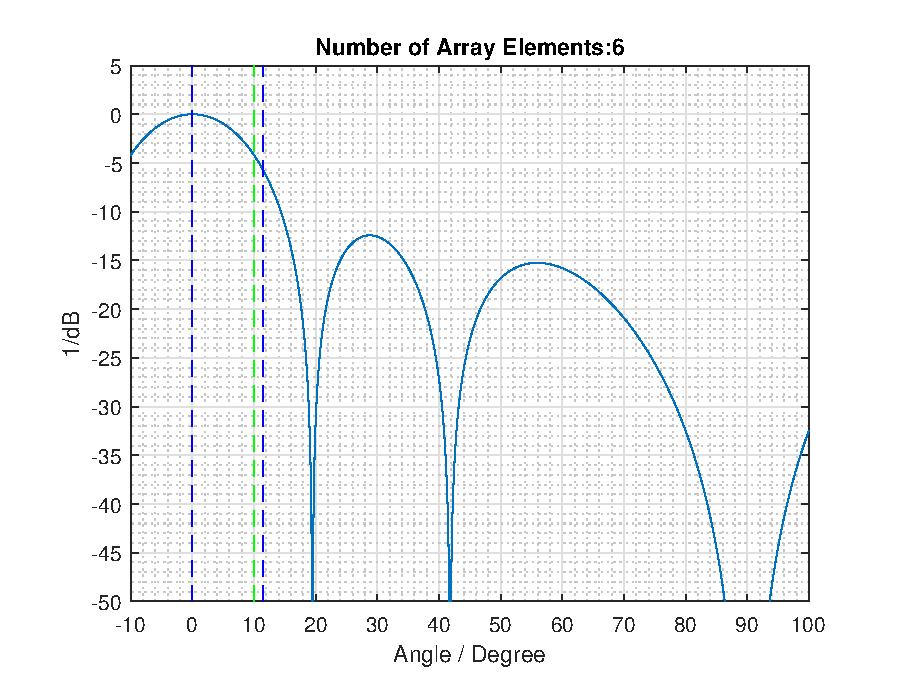
\includegraphics[width=0.32\textwidth]{Matlab/NoNumEl6.eps}}
  \centering
  \subfigure[100 elements: Pattern]{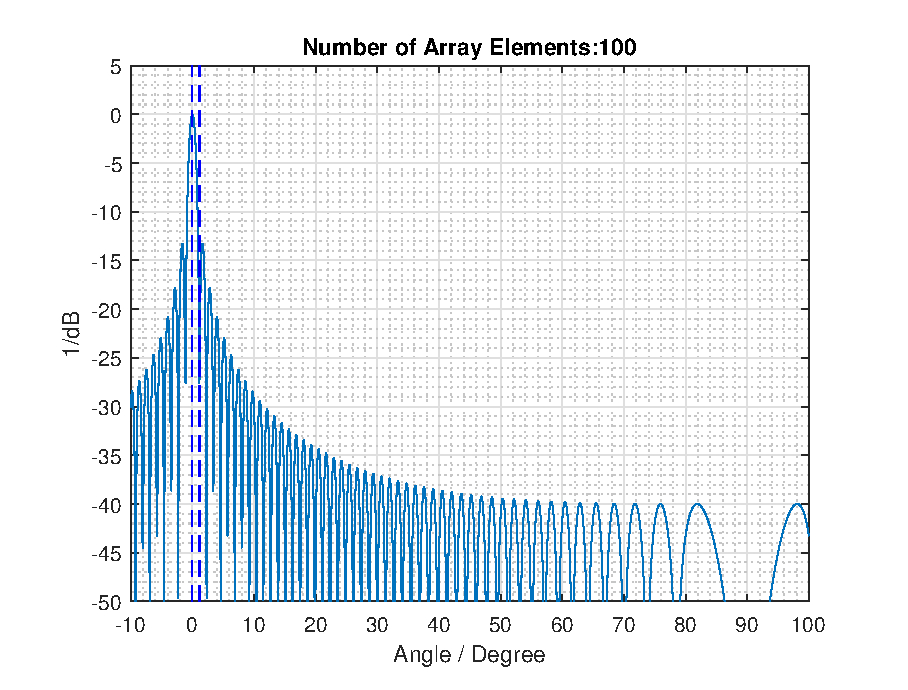
\includegraphics[width=0.32\textwidth]{Matlab/NoNumEl100.eps}}
\caption{Pattern of $N$-element array with $\sfrac{\lambda}{2}$-spacing}
\label{fig:evolvpattern2}
\end{figure}

The resulting pattern is depicted in figure \ref{fig:evolvpattern2} and in annex \ref{fig:evolvpattern} (a little larger).\\
In \cite{hansen} it is suggested to use the sampling increment of:

\begin{equation}
\Delta\Theta' = \frac{2\pi}{2N+1}\ , \quad \Delta\Phi'=\frac{2\pi}{2M+1}
\end{equation}

In which $N$ is the highest significant wave mode on the minimum sphere enclosing the antennas aperture and $M$ is the highest significant wave mode on the minimum cylinder. With the sphere radius $r_S$, the cylinder radius $r_C$ and the angular wavenumber $k = \sfrac{2\pi}{\lambda}$ they are calculated as follows:

\begin{equation}
N = kr_S+10\ , \quad M = kr_C+10
\end{equation}

The resulting formula is for example for the elevation:

\begin{equation}
\Delta\Theta_{\text{ref}} = \lim_{r_S \to \infty}\Delta\Theta' = \lim_{r_S \to \infty} \frac{2\pi}{2\left(kr_S+10\right)+1} = \frac{\lambda}{2\cdot r_S}
\end{equation}

Analogue to that in azimuth:

\begin{equation}
\Delta\Phi_{\text{ref}} = \frac{\lambda}{2\cdot r_C}
\end{equation}

These angle increments were also introduced in \cite{2018arXiv180310993F} and are called reference angle increments.

\begin{figure}
  \centering
  \subfigure[Two elements: Mode spectra]{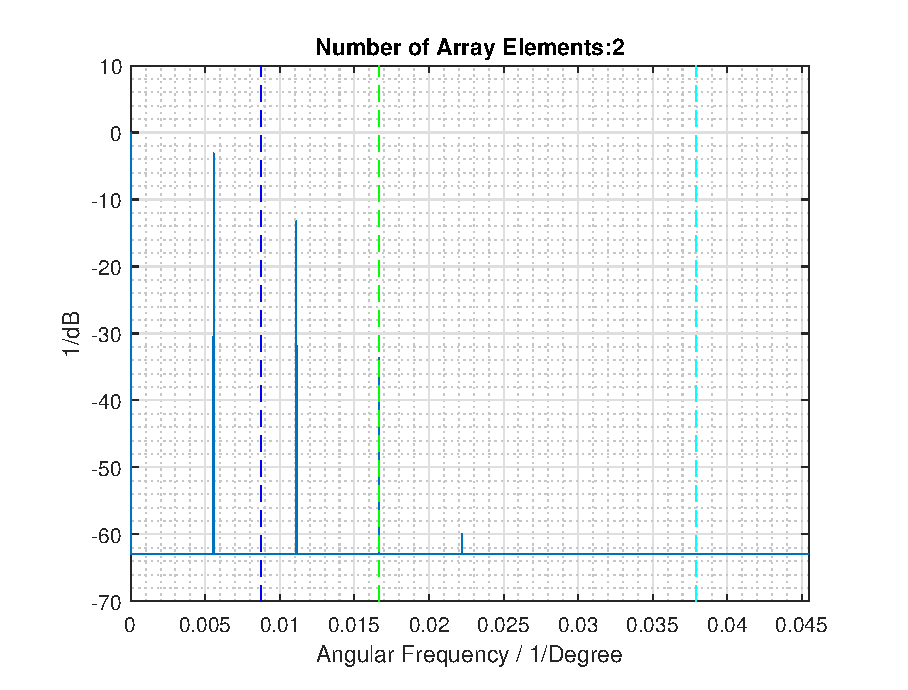
\includegraphics[width=0.32\textwidth]{Matlab/SpNumEl2.eps}}
  \centering
  \subfigure[Six elements: Mode spectra]{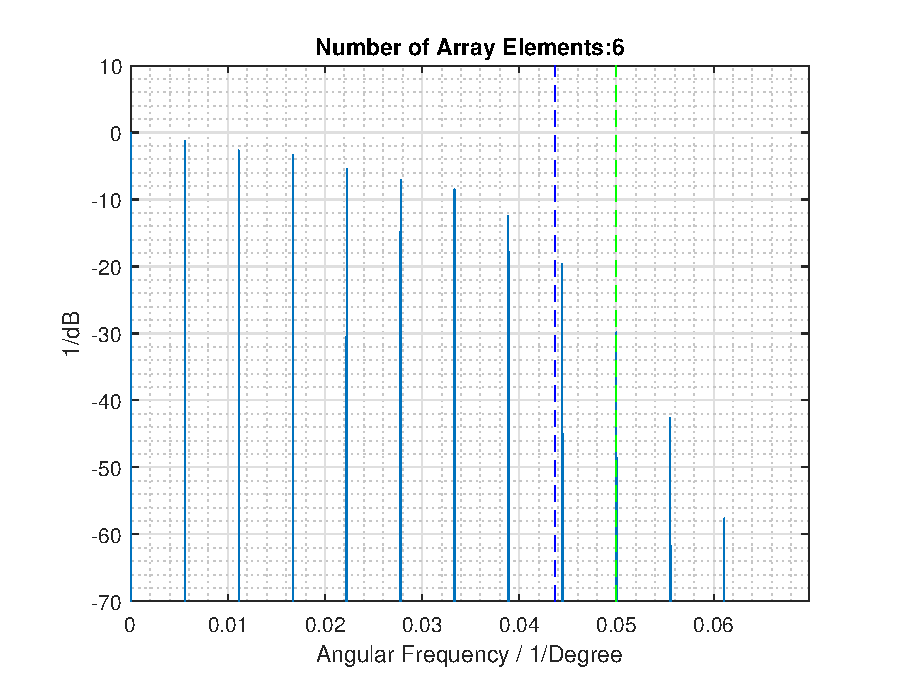
\includegraphics[width=0.32\textwidth]{Matlab/SpNumEl6.eps}}
  \centering
  \subfigure[100 elements: Mode spectra]{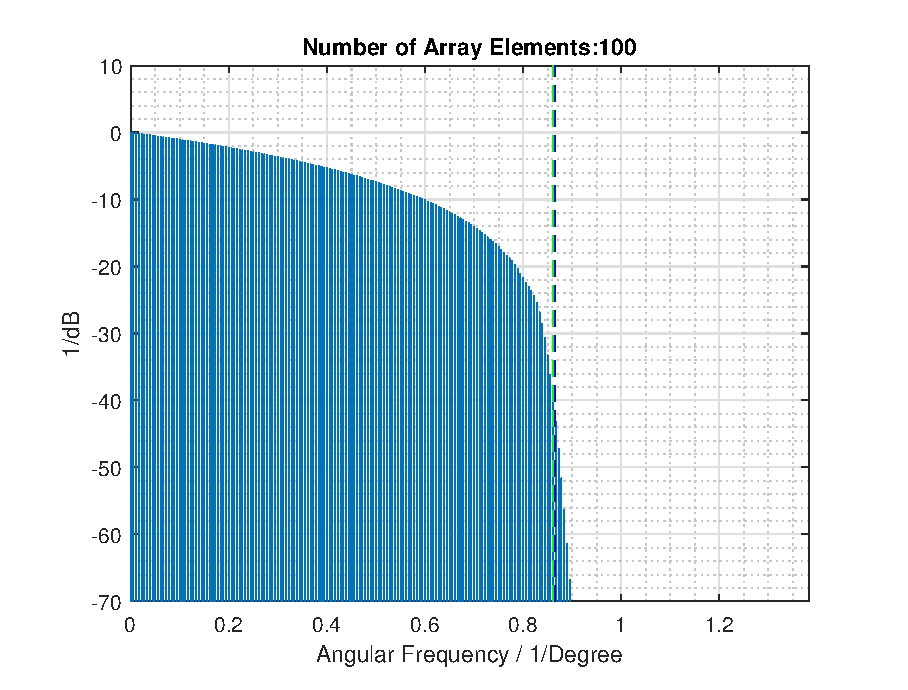
\includegraphics[width=0.32\textwidth]{Matlab/SpNumEl100.eps}}
\caption{Mode spectra of $N$-element array with $\sfrac{\lambda}{2}$-spacing}
\label{fig:evolvpattern3}
\end{figure}

To illustrate these angle increments the one dimensional array of isotropic radiators is taken. Evaluating the array factor of a $d = \sfrac{\lambda}{n}$ -array with $N$ elements the reference angel becomes very short:

\begin{equation}
\Delta\Phi_{\text{ref}} = \frac{n}{N-1}
\label{eq:1dinc}
\end{equation}

With the \ac{FFT} over the angle of the antenna patterns in figure \ref{fig:evolvpattern2} the mode spectra can be derived and is seen in figure \ref{fig:evolvpattern3} (or \ref{fig:evolvpattern} in annex).\\
When an arbitrary signal is sampled, the spectrum is mirrored at the sampling frequency. Choosing a sampling frequency lower than twice the highest occurring frequency in the sampled signal causes an irretrievable error. This is called the Nyquist-Shannon sampling theorem.\\
For that sake the dashed lines are:

\begin{equation}
\color{blue}\left(\Delta\Phi_{\text{ref}}\right)^{-1}\color{black},\ \color{cyan}\left(\Delta\Phi'\right)^{-1}\color{black}\ \text{and}\ \color{green}\text{first mode} > \SI{-40}{\decibel} \color{black}
\end{equation}

Similar to that the dashed lines in figure \ref{fig:evolvpattern2} are the first sampling points using the derived sampling frequency.\\
The issue is now to find the sampling frequency that the sampling error is independent from the aperture of the antenna. As depicted in figure \ref{fig:evolvpattern3} the sampling frequency introduced by \cite{hansen} is to strict for small apertures. On the other hand the reference angle introduced by \cite{2018arXiv180310993F} is to inaccurate for small apertures. Because of that a new factor is taken:

\begin{equation}
\text{CrefA} = \frac{\Delta\Phi_{\text{ref}}\cdot\left(\text{first mode} > \SI{-40}{\decibel}\right)}{2}
\end{equation} 

\begin{figure}
\centering
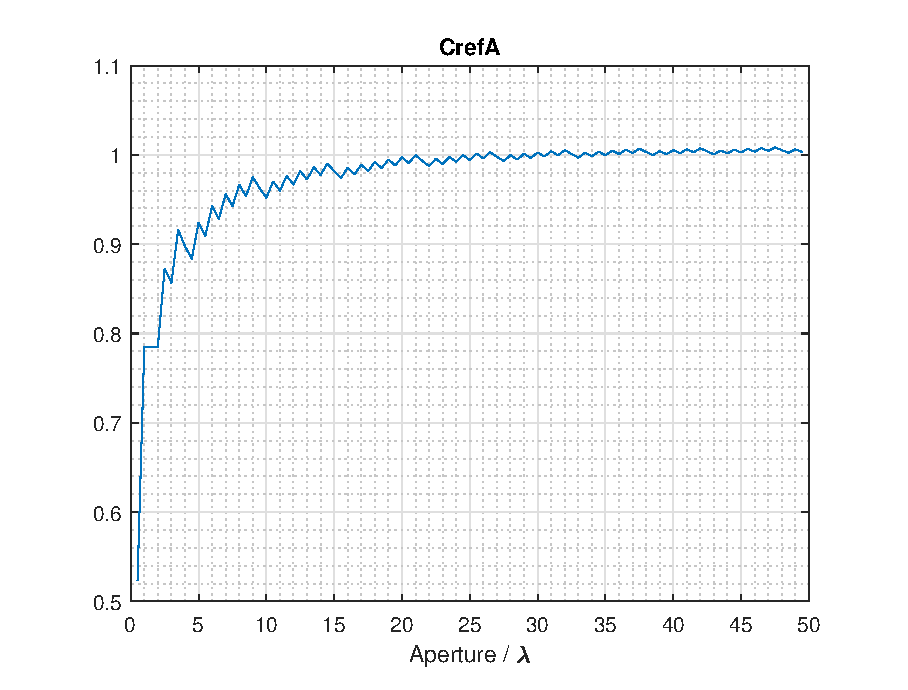
\includegraphics[width=0.41\textwidth]{Matlab/CrefA.eps}
\caption{Correction factor for reference angle}
\label{fig:crefa}
\end{figure}

This factor is plotted in figure \ref{fig:crefa}. It is dependent of the aperture. With that the error due to sampling is independent from the antennas aperture.\\
For further reduction of points a second factor is introduced, the Sparsity Factor SF. At $\text{SF}=2$ every second measurement point skipped. With all that the angle increments for spherical sampling is:

\begin{equation}
\Delta\Theta = \text{SF}\cdot\text{CrefA}\cdot\frac{\lambda}{2r_S}\ ,\quad\Delta\Phi = \text{SF}\cdot\text{CrefA}\cdot\frac{\lambda}{2r_C}
\end{equation}

\subsection{Constant Step Size Grid}


\begin{figure}[h]
  \centering
  \subfigure[without sinTF]{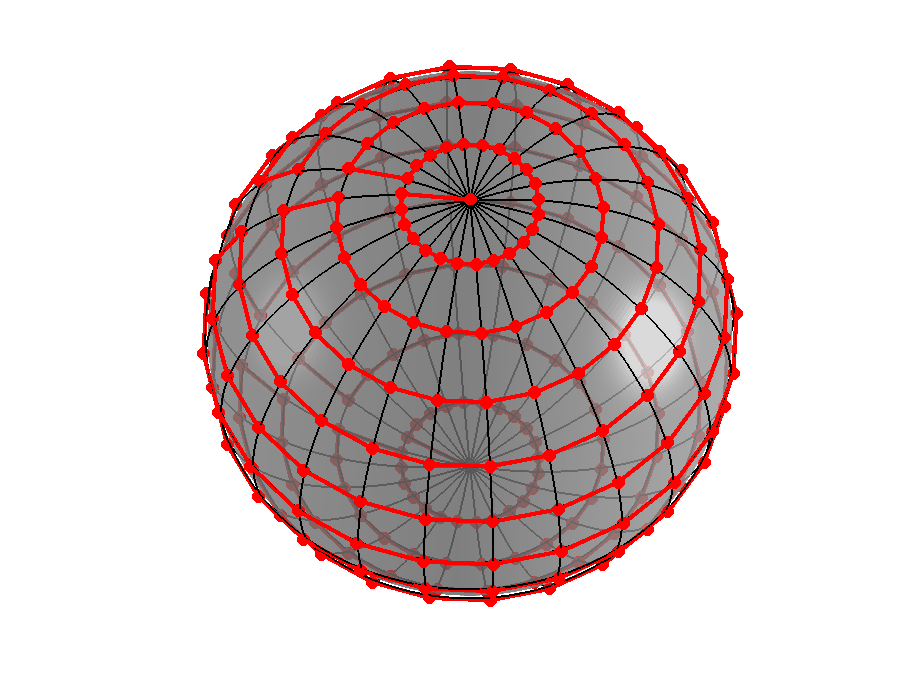
\includegraphics[width=0.49\textwidth]{Matlab/GridCoStPolar.eps}}
  \centering
  \subfigure[with sinTF]{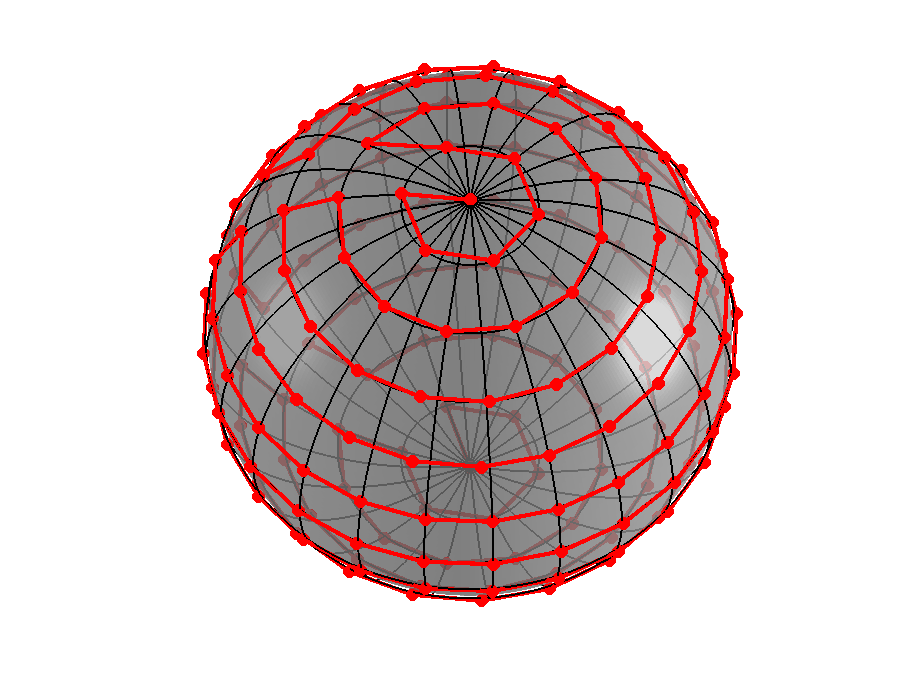
\includegraphics[width=0.49\textwidth]{Matlab/GridCoStSinPolar.eps}}
\caption{$\SI{15}{\degree}$ -Constant Step Size Grid}
\label{fig:cssg}
\end{figure}

The straight forward way to a spherical measurement is using a \ac{CSSG} depicted in figure \ref{fig:cssg} (a). The advantage is the easy feasibility with any positioner. Ether the azimuth can be sweep on every latitude circle or the elevation is swept on every longitude circle. On the other hand the measurement density is higher on the poles as on equator.\\
To meet that the theta dependent number of azimuth points was introduced e.g. by \cite{ctiaat}. It is applied as follows:

\begin{align}
N_{\text{max}} = \frac{2\pi}{\Delta\Phi}\\
N\left(\Theta\right)=\lceil N_{\text{max}}\cdot\cos\left(\Theta\right)\rceil\\
\Delta\Phi\left(\Theta\right) = \frac{2\pi}{N\left(\Theta\right)}
\end{align}

It is only possible to sweep the elevation when this type of grid is used.\\
For a better comparison of the grids, also in Cartesian presentation, which is interesting for the positioner, they are depicted in figure \ref{fig:gridcomp} in the annex. The red line is a suggested sequence.

\subsection{Constant Density}

\begin{figure}[h]
  \centering
  \subfigure[Polar Coordinates]{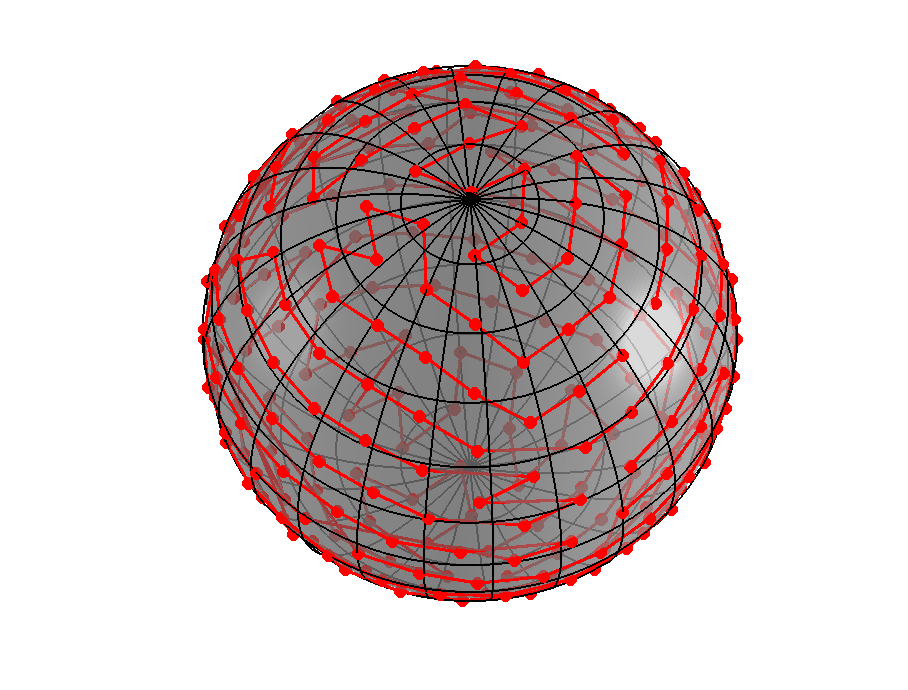
\includegraphics[width=0.49\textwidth]{Matlab/GridCoDePolar.eps}}
  \centering
  \subfigure[Cartesian Coordinates]{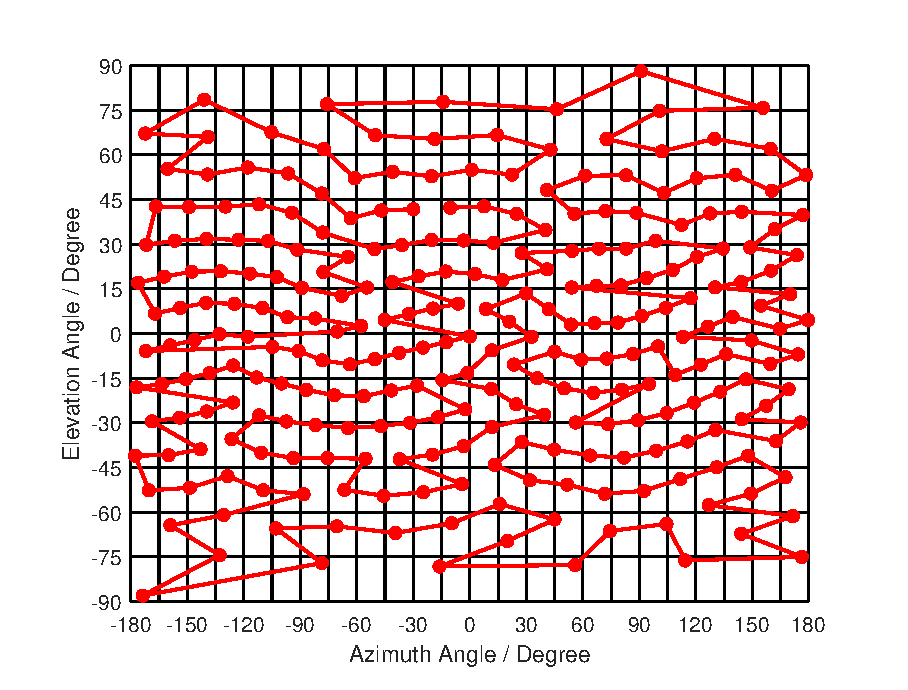
\includegraphics[width=0.49\textwidth]{Matlab/GridCoDeCart.eps}}
\caption{Constant Density Grid with 264 Measurementpoints}
\label{fig:cdg}
\end{figure}

The \ac{CDG} depicted in figure \ref{fig:cdg} was produces by a charged particle algorithm. It works by minimising the cumulated potential energy of all measurement dots considered as charged particles. The potential energy is minimal, when all points are evenly distributed over the sphere.\\ 
Deriving the optimal measurement sequence is a \ac{TSP}. It is solved by the Matlab toolbox introduced in \cite{tsp} viewing the angles as Cartesian coordinates. This is sensible for the positioner. Because the positioning in Azimuth is faster than in Elevation, the elevation distance is weighted five times more. Furthermore the periodicity is taken to account, so that the distance between tow points $\text{P}_n$ and $\text{P}_m$ is:

\begin{equation}
\Delta\Theta_{mn} = 5\left(\Theta_{\text{P}_n}-\Theta_{\text{P}_m}\right)\ ,\quad \Delta\Phi_{mn} = \text{min}\left(|\Phi_{\text{P}_n}-\Phi_{\text{P}_m}|\, ,\ 2\pi-|\Phi_{\text{P}_n}-\Phi_{\text{P}_m}|\right)
\end{equation}

With that the quadratic distance Matrix $D$ can be derived using euclidean distance with $d_{mn} = \sqrt{\Delta\Theta_{mn}^2+\Delta\Phi_{mn}^2}$ out of $N$ Points:

\begin{equation}
D = \begin{bmatrix}
 0 & d_{12} & \dots & d_{1N}\\
 d_{21} & 0 & \dots & d_{2N}\\
 \vdots & \vdots & \ddots & \vdots\\
 d_{N1} & d_{N2} & \dots & 0
\end{bmatrix}
\end{equation}

The cumulated distance for $N = 264$ is converged after around one million iterations. The result is depicted in figure \ref{fig:cdg} (b).

\subsection{Other}

Spiral Scan
Cardinal Cuts with or without Pattern Multiplication

\section{Total Radiated Power Integrals in Comparison}

\subsection{Sinus Theta}

\subsection{Jacobi}

\subsection{Clenshaw-Curtis}

\section{Statistics and Regression}